\documentclass[times, 10pt,twocolumn]{article}
\usepackage{latex8}
\usepackage{times}
\usepackage{psfig}

\usepackage{etex}
\usepackage[utf8]{inputenc}

\usepackage[left=1.00in,top=1.00in,bottom=1.00in,right=1.00in]{geometry}
\renewcommand{\baselinestretch}{1.00}
\pagestyle{empty}

\usepackage[%
    backend=biber,
    style=ieee,
    % style=numeric-comp,
    % style=numeric-comp,  % numerical-compressed
    sorting=none,        % nty,nyt,nyvt,anyt,anyvt,ynt,ydnt,none
    sortcites=true,      % sort \cite{b a d c}: true,false
    block=none,          % space between blocks: none,space,par,nbpar,ragged
    indexing=false,      % indexing options: true,false,cite,bib
    citereset=none,      % don't reset cites
    isbn=false,          % print ISBN?
    url=true,            % print URL?
    doi=false,           % print DOI?
    natbib=true,         % natbib compatability
  ]{biblatex}

% Reduce the font size of the bibliography:
\renewcommand{\bibfont}{\normalfont\footnotesize}

\addbibresource{refs.bib}

\usepackage{adjustbox}
\usepackage{graphicx}
\usepackage{wrapfig}

\usepackage{subcaption}
\expandafter\def\csname ver@subfig.sty\endcsname{}

%-------------------------------------------------------------------------
\begin{document}
\title{
\vspace{-0.8in}
Autotuning OpenCL Workgroup Sizes
\vspace{-0.2in}
}
\author{Chris Cummins, Hugh Leather, University of Edinburgh
}

\vspace{-3em}
\maketitle
\vspace{-3em}
\thispagestyle{empty}

The physical limitations of microprocessor design have forced the
industry towards increasingly heterogeneous designs to extract
performance, with an an increasing pressure to offload traditionally
CPU based workloads to the GPU. This trend has not been matched with
adequate software tools; the popular languages OpenCL and CUDA provide
a very low level model with little abstraction above the
hardware. Programming at this level requires expert knowledge of both
the domain and the target hardware, and achieving performance requires
laborious hand tuning of each program. This has led to a growing
disparity between the availability of parallelism in modern hardware,
and the ability for application developers to exploit it.

The goal of this work is to bring the performance of hand tuned
heterogeneous code to high level programming, by incorporating
autotuning into \textit{Algorithmic Skeletons}. Algorithmic Skeletons
simplify parallel programming by providing reusable, high-level,
patterns of computation. However, achieving performant skeleton
implementations is a difficult task; skeleton authors must attempt to
anticipate and tune for a wide range of architectures and use
cases. This results in implementations that target the general case
and cannot provide the performance advantages that are gained from
tuning low level optimization parameters for individual programs and
architectures. Autotuning offers promising performance benefits by
tailoring parameter values to individual cases, but the high cost of
searching the optimization space limits the practicality of autotuning
for real world programming~\cite{Ansel2013,Nugteren2015}. We believe
that performing machine learning-based autotuning at the skeletal
level of the can overcome these issues.

In this work, we present \textit{OmniTune} --- an extensible and
distributed framework for autotuning optimization parameters in
algorithmic skeletons at runtime. OmniTune enables a collaborative
approach to performance tuning, in which machine learning training
data is shared across a network of cooperating systems, amortizing the
cost of exploring the optimization space. We demonstrate the
practicality of OmniTune by autotuning the OpenCL workgroup size of
stencil skeletons in SkelCL. SkelCL~\cite{Steuwer2011} is an
Algorithmic Skeleton framework which abstracts the complexities of
OpenCL programming, exposing a set of data parallel skeletons for high
level heterogeneous programming in C++. Selecting an appropriate
OpenCL workgroup size is critical for the performance of programs, and
requires knowledge of the underlying hardware
(Figure~\ref{fig:motivation-arch}), the data being operated on, and
the program implementation (Figure~\ref{fig:motivation-prog}).

\begin{figure}
\centering
\adjustbox{valign=t}{%
  \begin{minipage}{.48\textwidth}
    \centering
    \begin{subfigure}[h]{.48\columnwidth}
      \centering
      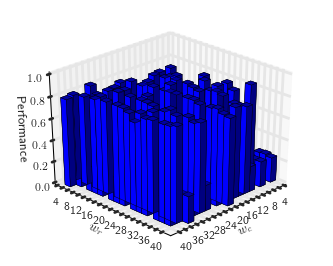
\includegraphics[width=1.0\columnwidth]{motivation_1}
      \vspace{-2em} % Shrink vertical padding
      \caption{}
      \label{fig:motivation-1}
    \end{subfigure}
    ~%
    \begin{subfigure}[h]{.48\columnwidth}
      \centering
      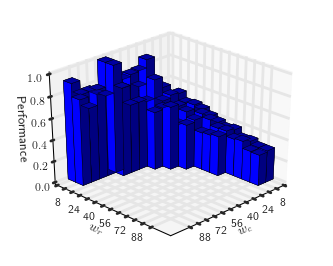
\includegraphics[width=1.0\columnwidth]{motivation_2}
      \vspace{-2em} % Shrink vertical padding
      \caption{}
      \label{fig:motivation-2}
    \end{subfigure}
    \caption{%
      Optimization space a single stencil on two different devices:
      (\subref{fig:motivation-1}) Intel CPU,
      (\subref{fig:motivation-2}) NVIDIA GPU.%
    }
    \label{fig:motivation-arch}
  \end{minipage}%
}%
\hspace{2.5mm}
\adjustbox{valign=t}{%
  \begin{minipage}{.48\textwidth}
    \centering
    \begin{subfigure}[h]{.48\columnwidth}
      \centering
      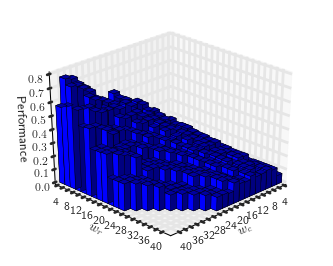
\includegraphics[width=1.0\columnwidth]{motivation_3}
      \vspace{-2em} % Shrink vertical padding
      \caption{}
      \label{fig:motivation-3}
    \end{subfigure}
    ~%
    \begin{subfigure}[h]{.48\columnwidth}
      \centering
      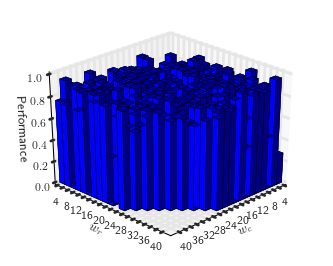
\includegraphics[width=1.0\columnwidth]{motivation_4}
      \vspace{-2em} % Shrink vertical padding
      \caption{}
      \label{fig:motivation-4}
    \end{subfigure}
    \caption{%
      Optimization space for a single device executing two different
      stencil programs.%
    }
    \label{fig:motivation-prog}
  \end{minipage}%
}
\vspace{-1.5em}
\end{figure}

Our autotuning approach employs the novel application of linear
regressors for classification of workgroup size, extracting 102
features at runtime describing the program, device, and dataset, and
predicting optimal workgroup sizes based on training data collected
using synthetically generated stencil benchmarks.

In an empirical study of 429 combinations of programs, architectures,
and datasets, we find that OmniTune provides a median $3.79\times$
speedup over the best possible fixed workgroup size, achieving 94\% of
the maximum performance. Our results demonstrate that autotuning at
the skeletal level --- when combined with sophisticated machine
learning techniques --- can raise the performance above that of human
experts, without requiring any effort from the user. By introducing
OmniTune and demonstrating its practical utility, we hope to
contribute toward increasing the programmability of heterogeneous
systems.

\vspace{-1em}
\printbibliography

\end{document}
